\documentclass[a4paper,12pt]{article} 
\usepackage[ngerman]{babel}
\usepackage{graphicx}
%\usepackage{amsmath}
\begin{document}

{\Large\bf Autonomes Automobil}

\medskip

Quentin Kniep, Timo Redweik, Nicolas Schmitt

\medskip

Friedrich-Wilhelm-Gymnasium K\"oln, Severinstr. 241, 50676 K\"oln

\medskip

5. April  2015

\medskip

{\bf  Abstract}
{\small We solve all problems. No questions remain.}

\medskip

{\bf  Zusammenfassung}
{\small Wir l\"osen alle Probleme. Es bleiben keine Fragen.}

\medskip

{\bf  Keywords:}
{\small Gl\"uck, Geld, Sorgenfreies Leben}

\bigskip


\section{Einf\"uhrung}\label{sec1}

Ziel unseres Projekts war es, ein Modellauto so zu programmieren, dass es selbst\"andig fahren und Hindernissen ausweichen kann.
Dazu haben wir einen Computer in das Auto eingebaut und diesen mit dem Motor verbunden.
Zus\"atzlich haben wir Ultraschallsensoren f\"ur die Abstandsmessung eingebaut.

Ein grundlegender Schaltplan ist in Abb.~\ref{Fig1} vereinfacht dargestellt.

\begin{figure}[h]
	\centering
	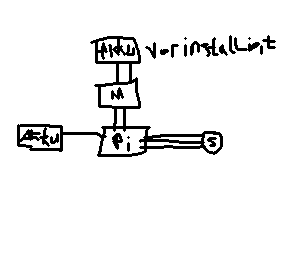
\includegraphics[width=6cm]{./media/Fig1.png}
	\caption{grundlegender Schaltplan}
	\label{Fig1}
\end{figure}

Die wichtigsten Teilaspekte haben wir in Tabelle~\ref{Tab1} zusammengefasst.

\begin{table}[h]
	\centering
	\begin{tabular}{|c|c|c|}
	\hline
		Gl\"uck & Geld  & Sorgenfreies Leben  \\ \hline
		Ja  & Ja & Jaja \\ \hline
	\end{tabular}
	\caption{Sinnfindung}
	\label{Tab1}
\end{table}


\section{Hauptteil}\label{sec2}

Zuerst haben wir das Problem analysiert und das Arbeitsprogramm erstellt.

\subsection{Hauptteil Unterabschnitt}\label{sec2.1}

Der erste Arbeitsunterpunkt wurde so behandelt und folgender L\"osung zugef\"uhrt.

\subsection{Hauptteil Unterabschnitt}\label{sec2.2}

Der zweite Arbeitsschritt f\"uhrte uns auf eine bezaubernde Gleichung

\begin{equation}
	E = mc^2 ,
\end{equation}

die der Kollege Albert vom Patentamt Bern  \cite{Alb05} auch schon beschrieben hat.


\section{Fazit und Ausblick}\label{sec3}

Alles hat wunderbar geklappt. Nichts ging schief und alle sind happy.


\bigskip


{\large\bf Danksagung}

\bigskip


{\large\bf Erkl\"arung der Eigenst\"andigkeit}

\bigskip


\begin{thebibliography}{99}
	\itemsep-2pt \small\frenchspacing
	\bibitem{Alb05}A. Einstein, Annalen der Physik {\bf 18}, 639 (1905).
	\newline
	\bibitem{Alb06}A. Einstein, Annalen der Physik {\bf 18}, 639 (1906).
\end{thebibliography}


\pagebreak

\subsection{Hauptteil Unterabschnitt}\label{sec2.2}

F\"ur die Steuerung des Autos haben wir ein Programm geschrieben, welches auf dem, von uns im Auto eingebauten,
Raspberry Pi ausgef\"uhrt wird. Bei der Auswahl der Programmiersprache konnten wir uns, auf Grund unseres Vorwissens und der
technischen Limitierung des Raspberry Pi, lediglich zwischen Python und C++ entscheiden. Wir haben uns dabei dann f\"ur
Python entschieden. Vorallem auf Grund der einfachen Syntax, welche uns schnellere \"Anderungen am Programm-Code erlaubt.
\newline
Die grundlegende Aufgabe des Programms ist es zuerst Messungen, mittels der Ultraschallsensoren durchzuf\"uhren, diese
Messungen auszuwerten, und dann entsprechende Signale an die Motoren des Autos zu senden.

\medskip

Zuerst definieren wir ein paar Konstanten, die in dem Programm h\"aufiger verwendet werden, etwa den Umrechnungsfaktor mit
dem wir aus der Zeit, die das Ultraschallsignal braucht, die Enfernung des Objektes berechnen k\"onnen und umgekehrt.
Diesen Wert haben wir zuerst durch einen einfachen Versuch herausfinden m\"ussen. Wir haben Objekte in bestimmten
Entfernungen des Autos gestellt, und Messungen durchgef\"uhrt. Dies haben wir f\"ur Objekte in verschiedenen Entfernungen
durchgef\"uhrt, sodass wir schlie"slich durch den Quotienten aus Strecke und Zeit den Umrechnungsfaktor errechnen konnten
Oder auch die von uns festgelegte maximale Abweichung die ein Wert haben darf ohne als Fehlerwert zu gelten. Und auch
die Nummern der von uns verwendeten Pins am Raspberry Pi speichern wir in Konstanten, damit wir diese nachher einfacher
abrufen k\"onnen und die jeweilige Zahl nur ein einziges mal im Code vorkommt. Somit muss bei einem Umstecken der
Verbindungen nur eine Zahl ge\"andert werden.
\newline
Au"serdem deklarieren wir einige Variablen, die wir verwenden k\"onnen um w\"ahrend der Ausf\"uhrung des Programms Werte
zwischenzuspeichern. Die wichtigsten eieser Variablen sind unsere vier Listen. In der Liste RESULT speichern wir die
letzten Werte, die die Ultraschallsensoren gemessen haben, das hei"st die Zeiten zwischen Senden des Ultraschallsignals
und erneuten Empfangen desselben, und den dazugeh\"origen Zeitpunkt, zu dem die Messung stattgefunden hat. In dieser
Liste sind immer nur die letzten Messwerte gespeichert, bis sie auf Fehler \"uberpr\"uft wurden. Wenn sie nach der
\"Uberpr\"ufung als Fehlerwert gelten, d.h. eine zu gro"se Abweichung von dem vorigen Messwert haben, kommen sie in
unsere Liste WDATA. In dieser werden die Werte dann erneut f\"ur eine weitere \"Uberpr\"ufung zwischengespeichert. Bei
dieser werden die letzten Messwerte je mit den Werten aus der vierten Liste verglichen. Das hei"st es wird letztendlich
\"uberpr\"uft ob sich die letzten Messwerte, nachdem ein Fehler erkannt wurde, stark genug \"ahneln um doch als richtige
Werte zu gelten. Sobald die Werte nach einer \"Uberpr\"ufungen als richtige Werte angesehen werden, werden die Messwerte
in die Liste DATA \"uberf\"uhrt und die dazugeh\"origen Zeitpunkte in die Liste TIME. Die Werte aus diesen beiden Listen
k\"onnenn letztendlich in Entfernungen umgerechnet werden und so weiterhin verwendet werden, etwa f\"ur die Berechnung der
Geschwindigkeit oder f\"ur das Einleiten eines Bremsvorganges, wenn das Hindernis dem Auto zu nahe kommt. Auf Grund von
Fehlerwerten, die nicht als Messwerte aufgennommen werden, sind die Messungen nicht zwangsl\"aufig in gleichm\"a"sigen
Zeitabst\"anden. In diesen F\"allen wird der Zeitpunkt der Messung ben\"otigt um bestimmte Berechnungen, wie etwa die
Errechnung der Geschwindigkeit, durchzuf\"uhren.

\medskip

Beim Ausf\"uhren des Programms wird zuerst unsere Hauptmethode aufgerufen, innerhalb dieser werden dann der Reihe nach
einige spezialisierte Funktionen aufgerufen, welche sich jeweils mit einem Arbeitsschritt befassen. Etwa die Methode
measure(i), welche eine Messung mit dem Sensor i durchf\"uhrt und das Ergebnis abspeichert. Wobei i die Nummer des
Sensors ist (wir haben diese von 0 bis 3 durchnummeriert). Diese Funktionen werde ich im Folgenden einzeln
erl\"autern.

\medskip

\textbf{setup()}
\newline
Diese Funktion wird als erstes ausgef\"uhrt wenn das Hauptprogramm gestartet wird. Sie ist daf\"ur zust\"andig alle Pins
wieder auf ihren Ausgangszustand zur\"uckzusetzen, d.h. die Pins auf OUT bzw. IN zu stellen und die angelegte Spannung
der OUT-Pins auf 0V zu setzen. Au"serdem werden die Einstellungen der GPIO Library gesetzt. Die GPIO Library haben wir
als Schnittstelle zwischen unserem Programm und den Pins des Raspberry Pi gew\"ahlt. Durch Funktionsaufrufe an diese
Library k\"onnen wir ablesen ob an den IN-Pins eine Spannung von 3,5 V anliegt und wir k\"onnen an den OUT-Pins selbst
eine Spannung von 3,5 V anlegen.

\medskip

\textbf{driveForward()}
\newline
Beim Aufruf dieser Funktion f\"angt das Auto anzufahren. Dies wird durch eine \"Anderung der Spannungen an den Pins, die
\"uber das Relay am Antriebsmotor angeschlossen sind, erreicht. Diese \"Anderung sorgt letztendlich daf\"ur, dass ein
geschlossener Stromkreis zwischen dem Akku des Autos und dem Antriebsmotor entsteht, und dass eine positive Spannung an
diesem anliegt, was daf\"ur sorgt, dass das Auto beginnt vorw\"arts zu beschleunigen.

\medskip

\textbf{measure(i)}
\newline
Der Parameter i in dieser Funktion beschreibt den Sensor, mit dem gemssen werden soll. Dabei handelt es sich bei i um
eine Zahl von 0 bis 3. Zuerst f\"uhrt diese Funktion eine Messung mit dem angegebenen Sensor durch. Danach wird der
erhaltene Messwert in der Liste RESULT abgespeichert. Um eine Messung mit dem Ultraschallsensor zu starten muss man
diesem zuerst \"uber den daran angeschlossenen OUT-Pin einen elektrischen Impuls, der Dauer 10 µs und Spannung 3,5 V, 
geben. Dann wartet unser Programm auf eine R\"uckmeldung durch den Sensor, dies Erfolgt durch einen \"ahnlichen
elektrischen Impuls, den wir \"uber den IN-Pin, der mit dem Sensor verbunden ist, empfangen k\"onnen. Den Zeitpunkt zu
dem wir diesen Impuls empfangen haben speichern wir zwischen. Da dieser genau dem Zeitpunkt entspricht zu dem das
Ultraschallsignal gesendet wurde. Entsprechend dem ersten kommt dann, bei Empfangen des Ultraschallsignals, ein weiterer
Impuls, den wir erneut empfangen und dessen Zeitpunkt abspeichern. Sodass wir schlie"slich durch die Differenz der
beiden Zeitpunkte die Zeit herausfinden, die das Ultraschallsignal gebraucht hat, f\"ur Hin- und R\"uckweg. Hierbei
haben wir au"serdem einen Schutz eingebaut, der das Programm davor sch\"utzt in einer Messung unendlich lang auf den
zweiten Impuls zu warten. Und zwar wird das Warten auf den zweiten Impuls nach 25 ms abgebrochen. Falls dies passiert,
wird als gemessener Zeitwert -1 abgespeichert, dies behandeln wir im Programm allgemein als fehlgeschlagene Messungen.

\medskip

\textbf{check\_results(i)}
\newline
Bereits bei den ersten Tests ist uns aufgefallen, dass relativ h\"aufig fehlerhafte Werte auftreten. Deshalb war uns
schon ziemlich fr\"uh klar, dass wir eine Funktion brauchen, die die Messwerte auf ihre Richtigkeit \"uberpr\"uft.

\end{document}
